\documentclass[9pt, handout]{beamer}
\usetheme{CambridgeUS}
\usepackage{xcolor}
\usepackage{geometry}
\usepackage{array}
\usepackage{comment}

\AtBeginSection[]
{
  \begin{frame}
    \frametitle{Table of Contents}
    \tableofcontents[currentsection]
  \end{frame}
}

\setbeamertemplate{footline}
{
  \leavevmode%
  \hbox{%
    \begin{beamercolorbox}[wd=.333333\paperwidth,ht=2.25ex,dp=1ex,center]{author in head/foot}%
      \usebeamerfont{author in head/foot}\insertshortauthor
    \end{beamercolorbox}%
    \begin{beamercolorbox}[wd=.333333\paperwidth,ht=2.25ex,dp=1ex,center]{title in head/foot}%
      \usebeamerfont{title in head/foot}\insertshortsubtitle
    \end{beamercolorbox}%
    \begin{beamercolorbox}[wd=.333333\paperwidth,ht=2.25ex,dp=1ex,right]{date in head/foot}%
      \usebeamerfont{date in head/foot}\insertshortdate{}\hspace*{2em}
      \usebeamertemplate{page number in head/foot}\hspace*{2ex}
    \end{beamercolorbox}
  }%
  \vskip0pt%
}

\title{Principles of Economics}
\subtitle{Discussion Session 4: Evaluating Welfare}
\author{Joe Wilske}
\institute{Boston College}
\date{\today}

\begin{document}

\frame{\titlepage}

\begin{frame}{Consumer Surplus}
    \begin{itemize}
        \item \textbf{Consumer Surplus} is the difference between a consumer's willingness to pay and the actual price paid.
        \item The ``surplus'' value one gets from purchasing a good.
    \end{itemize}
    \begin{figure}
        \centering
        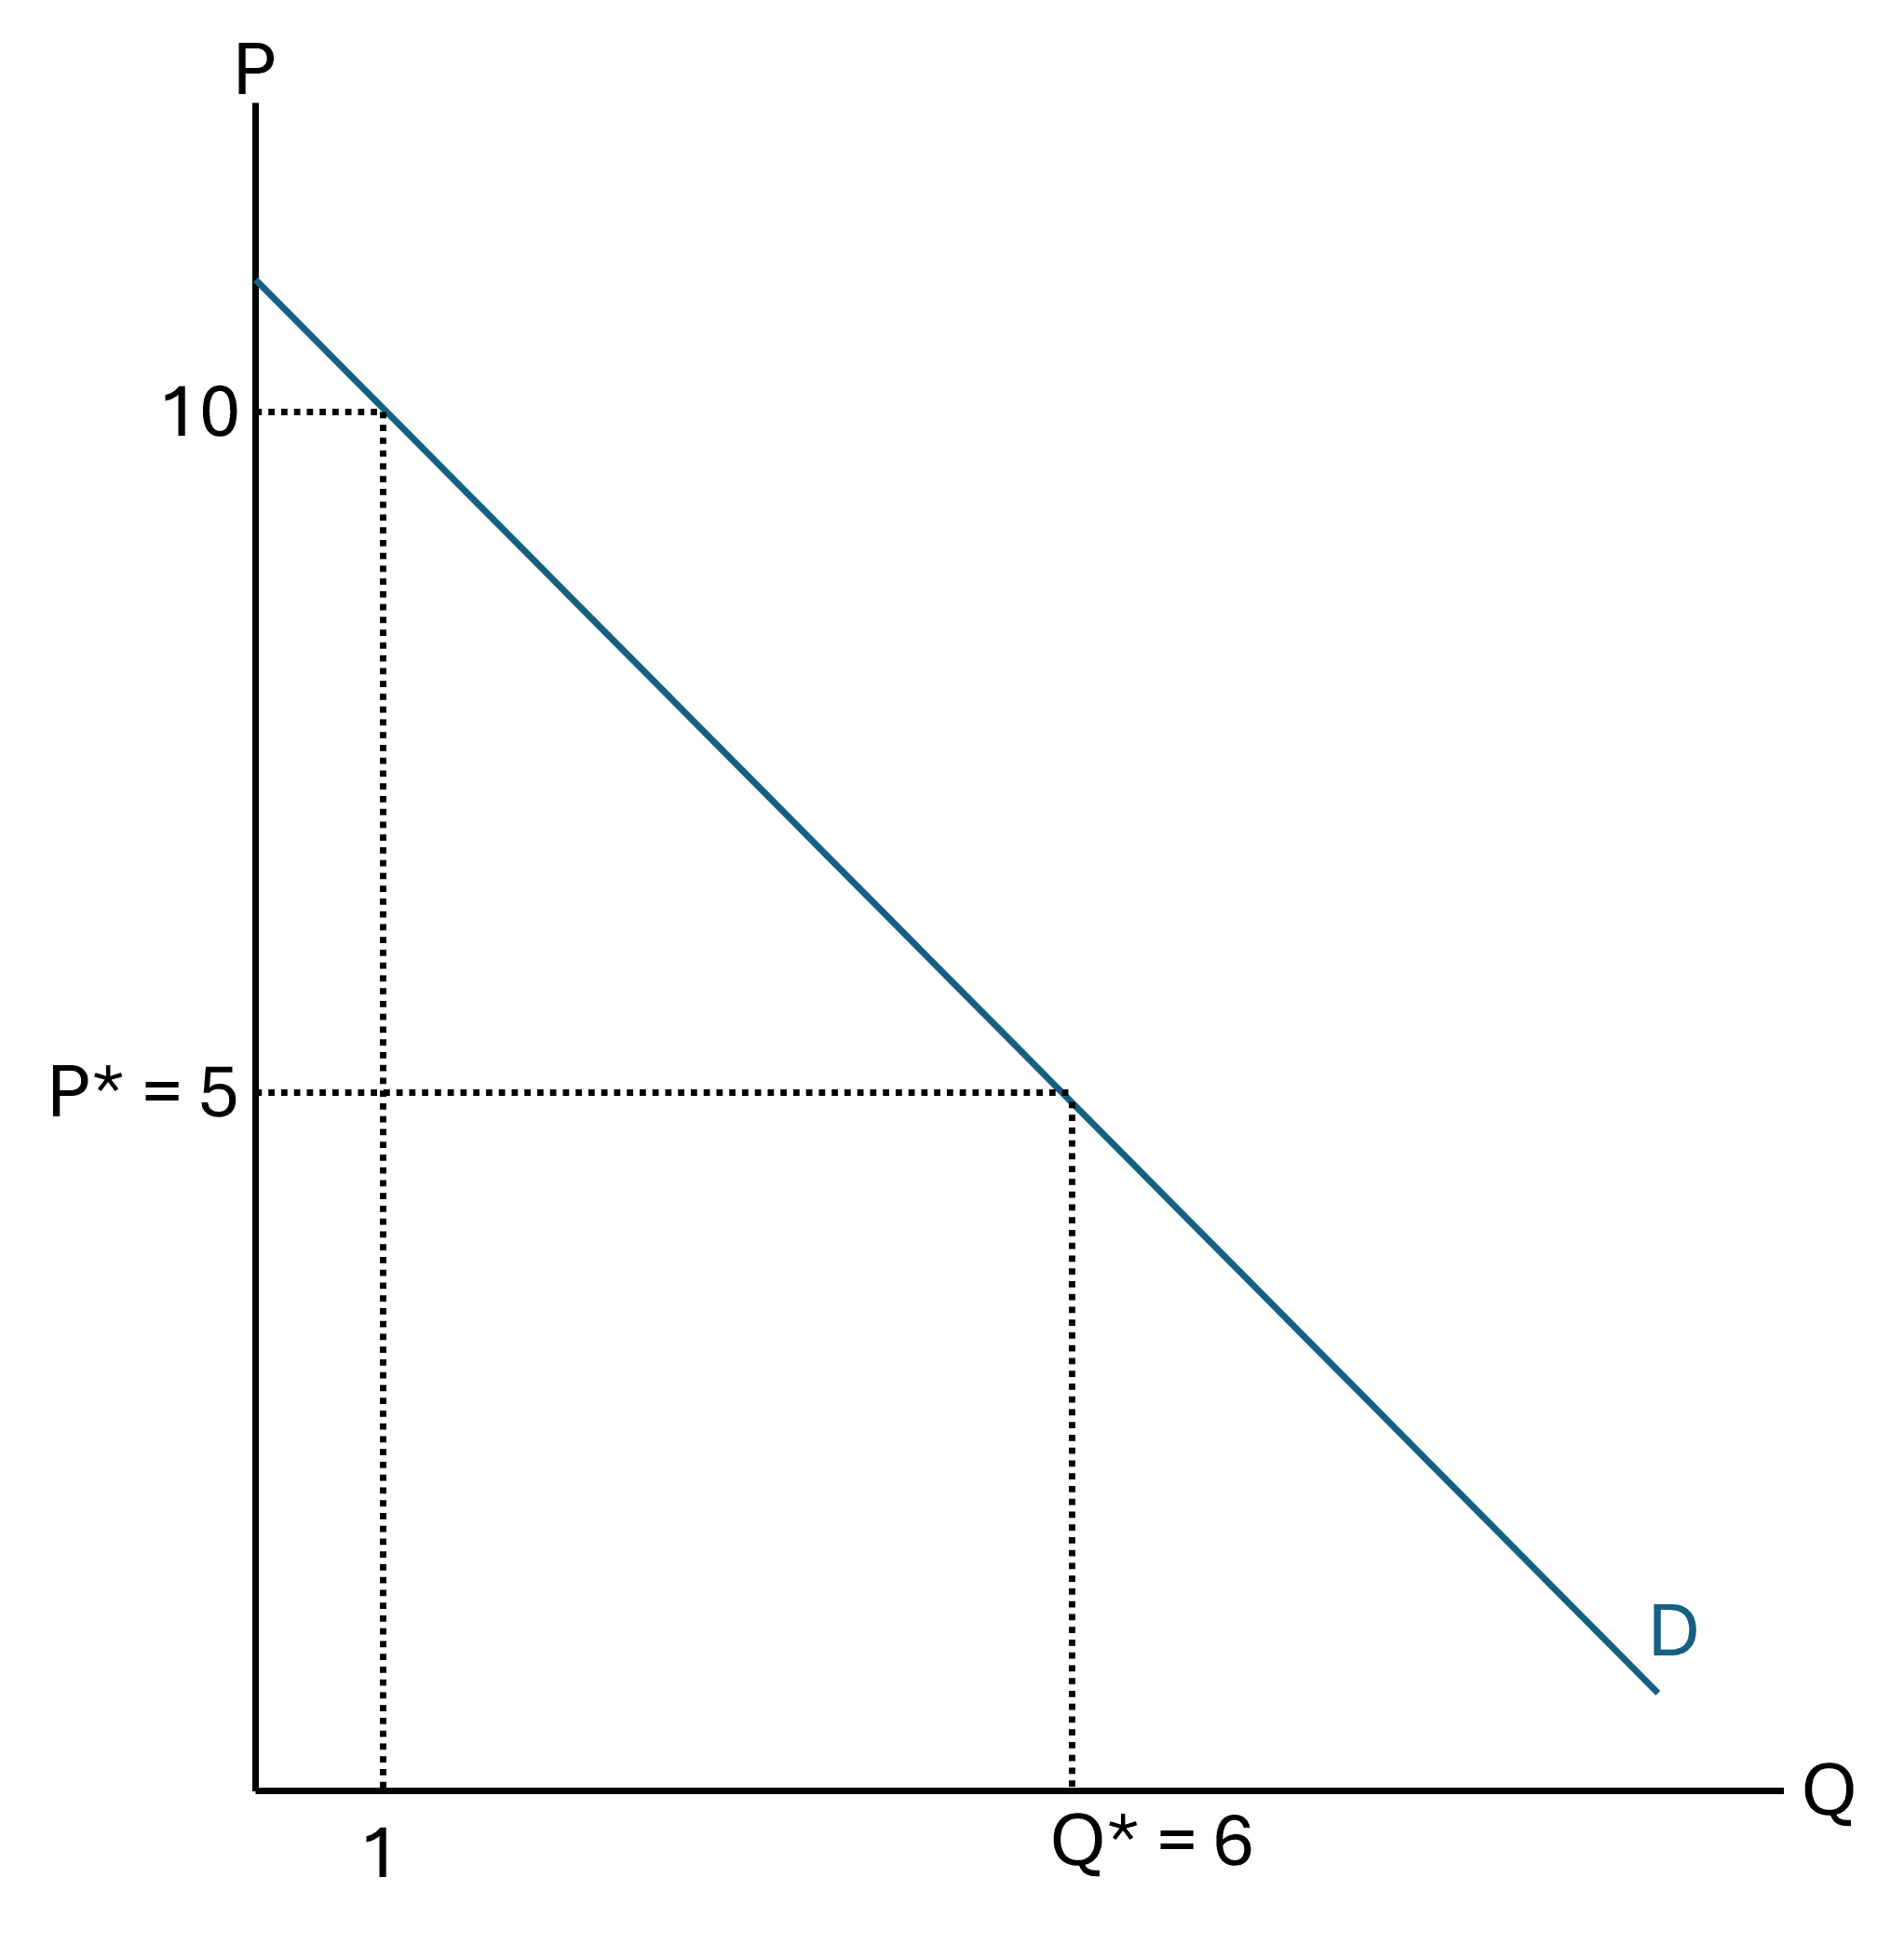
\includegraphics[width=0.4\linewidth]{Picture1.png}
    \end{figure}
    \begin{itemize}
        \item This consumer is willing to pay \$10 for one unit.
        \item Since the market price is \$5, he gets $\$10 - \$5 = \$5$ of surplus value from that unit.
    \end{itemize}
\end{frame}

\begin{frame}{Consumer Surplus: Continued}
    \begin{itemize}
        \item Adding together the surplus from every unit purchased gives the total CS.
        \item Calculated by finding the area between the demand curve and price paid.
    \end{itemize}
    \begin{figure}
        \centering
        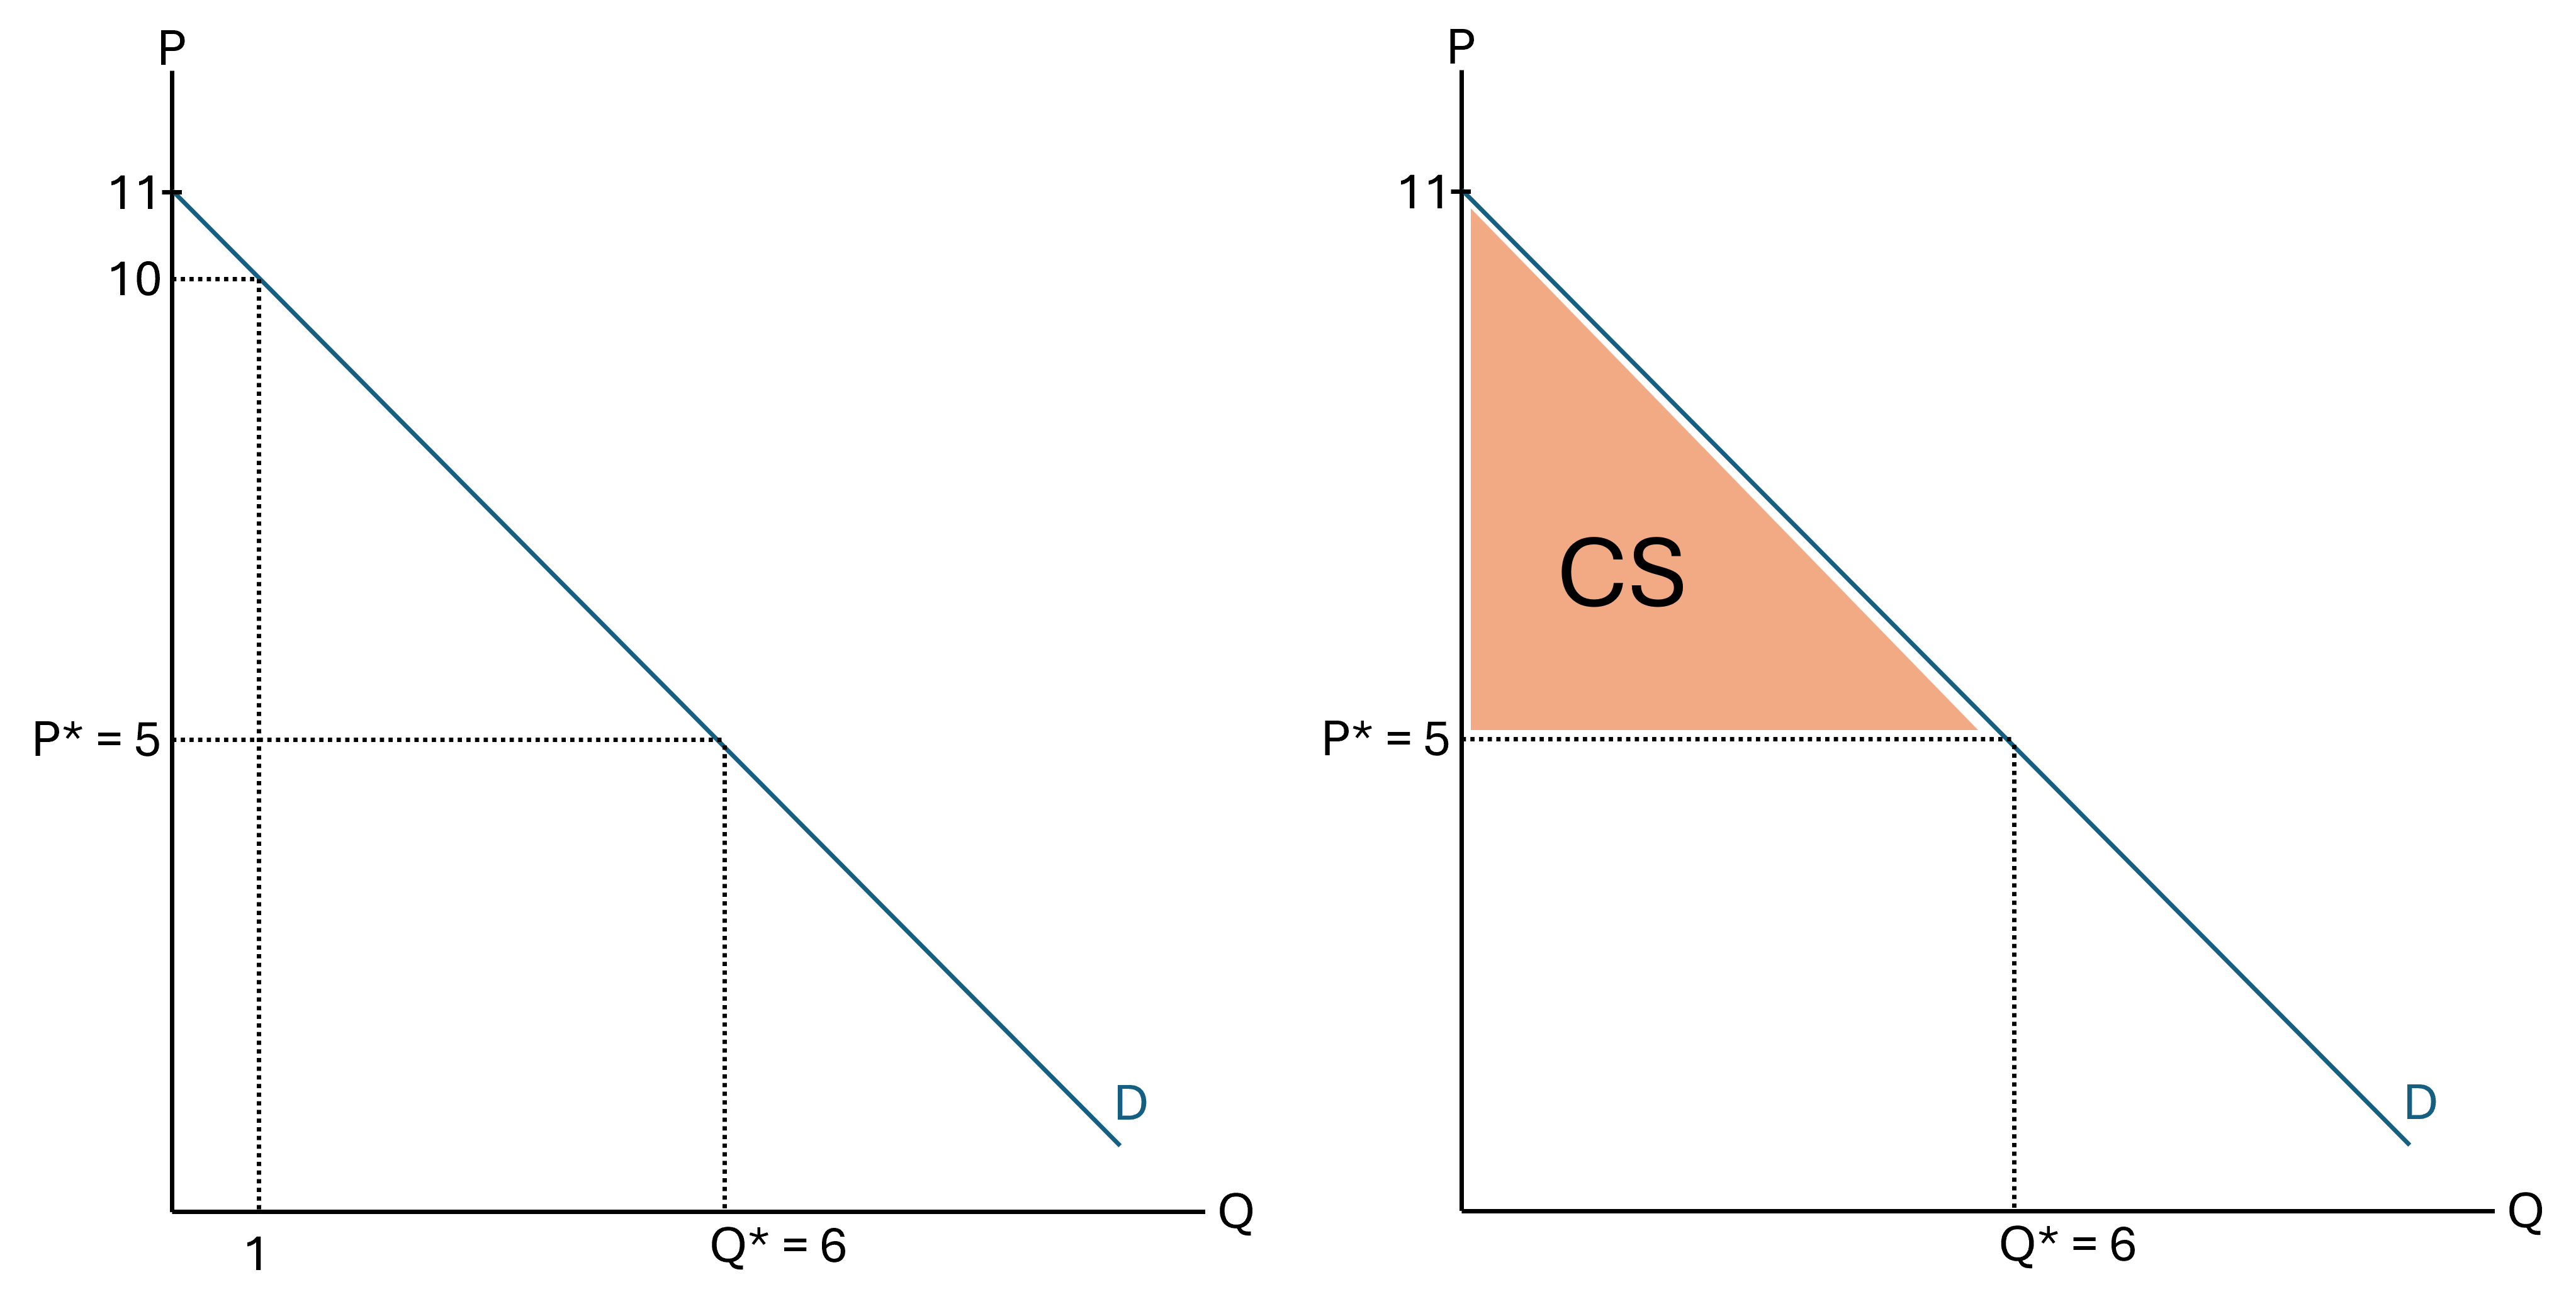
\includegraphics[width=.85\linewidth]{Picture2.png}
    \end{figure}
    \begin{itemize}
        \item $CS = \frac{1}{2}bh = \frac{1}{2}(6)(6) = 18$
    \end{itemize}
\end{frame}

\begin{frame}{Producer Surplus}
    \begin{itemize}
        \item \textbf{Producer Surplus} is the difference between the actual price received and a producer's willingness to sell.
        \item Calculated by finding the area between the supply curve and price received.
    \end{itemize}
    \begin{figure}
        \centering
        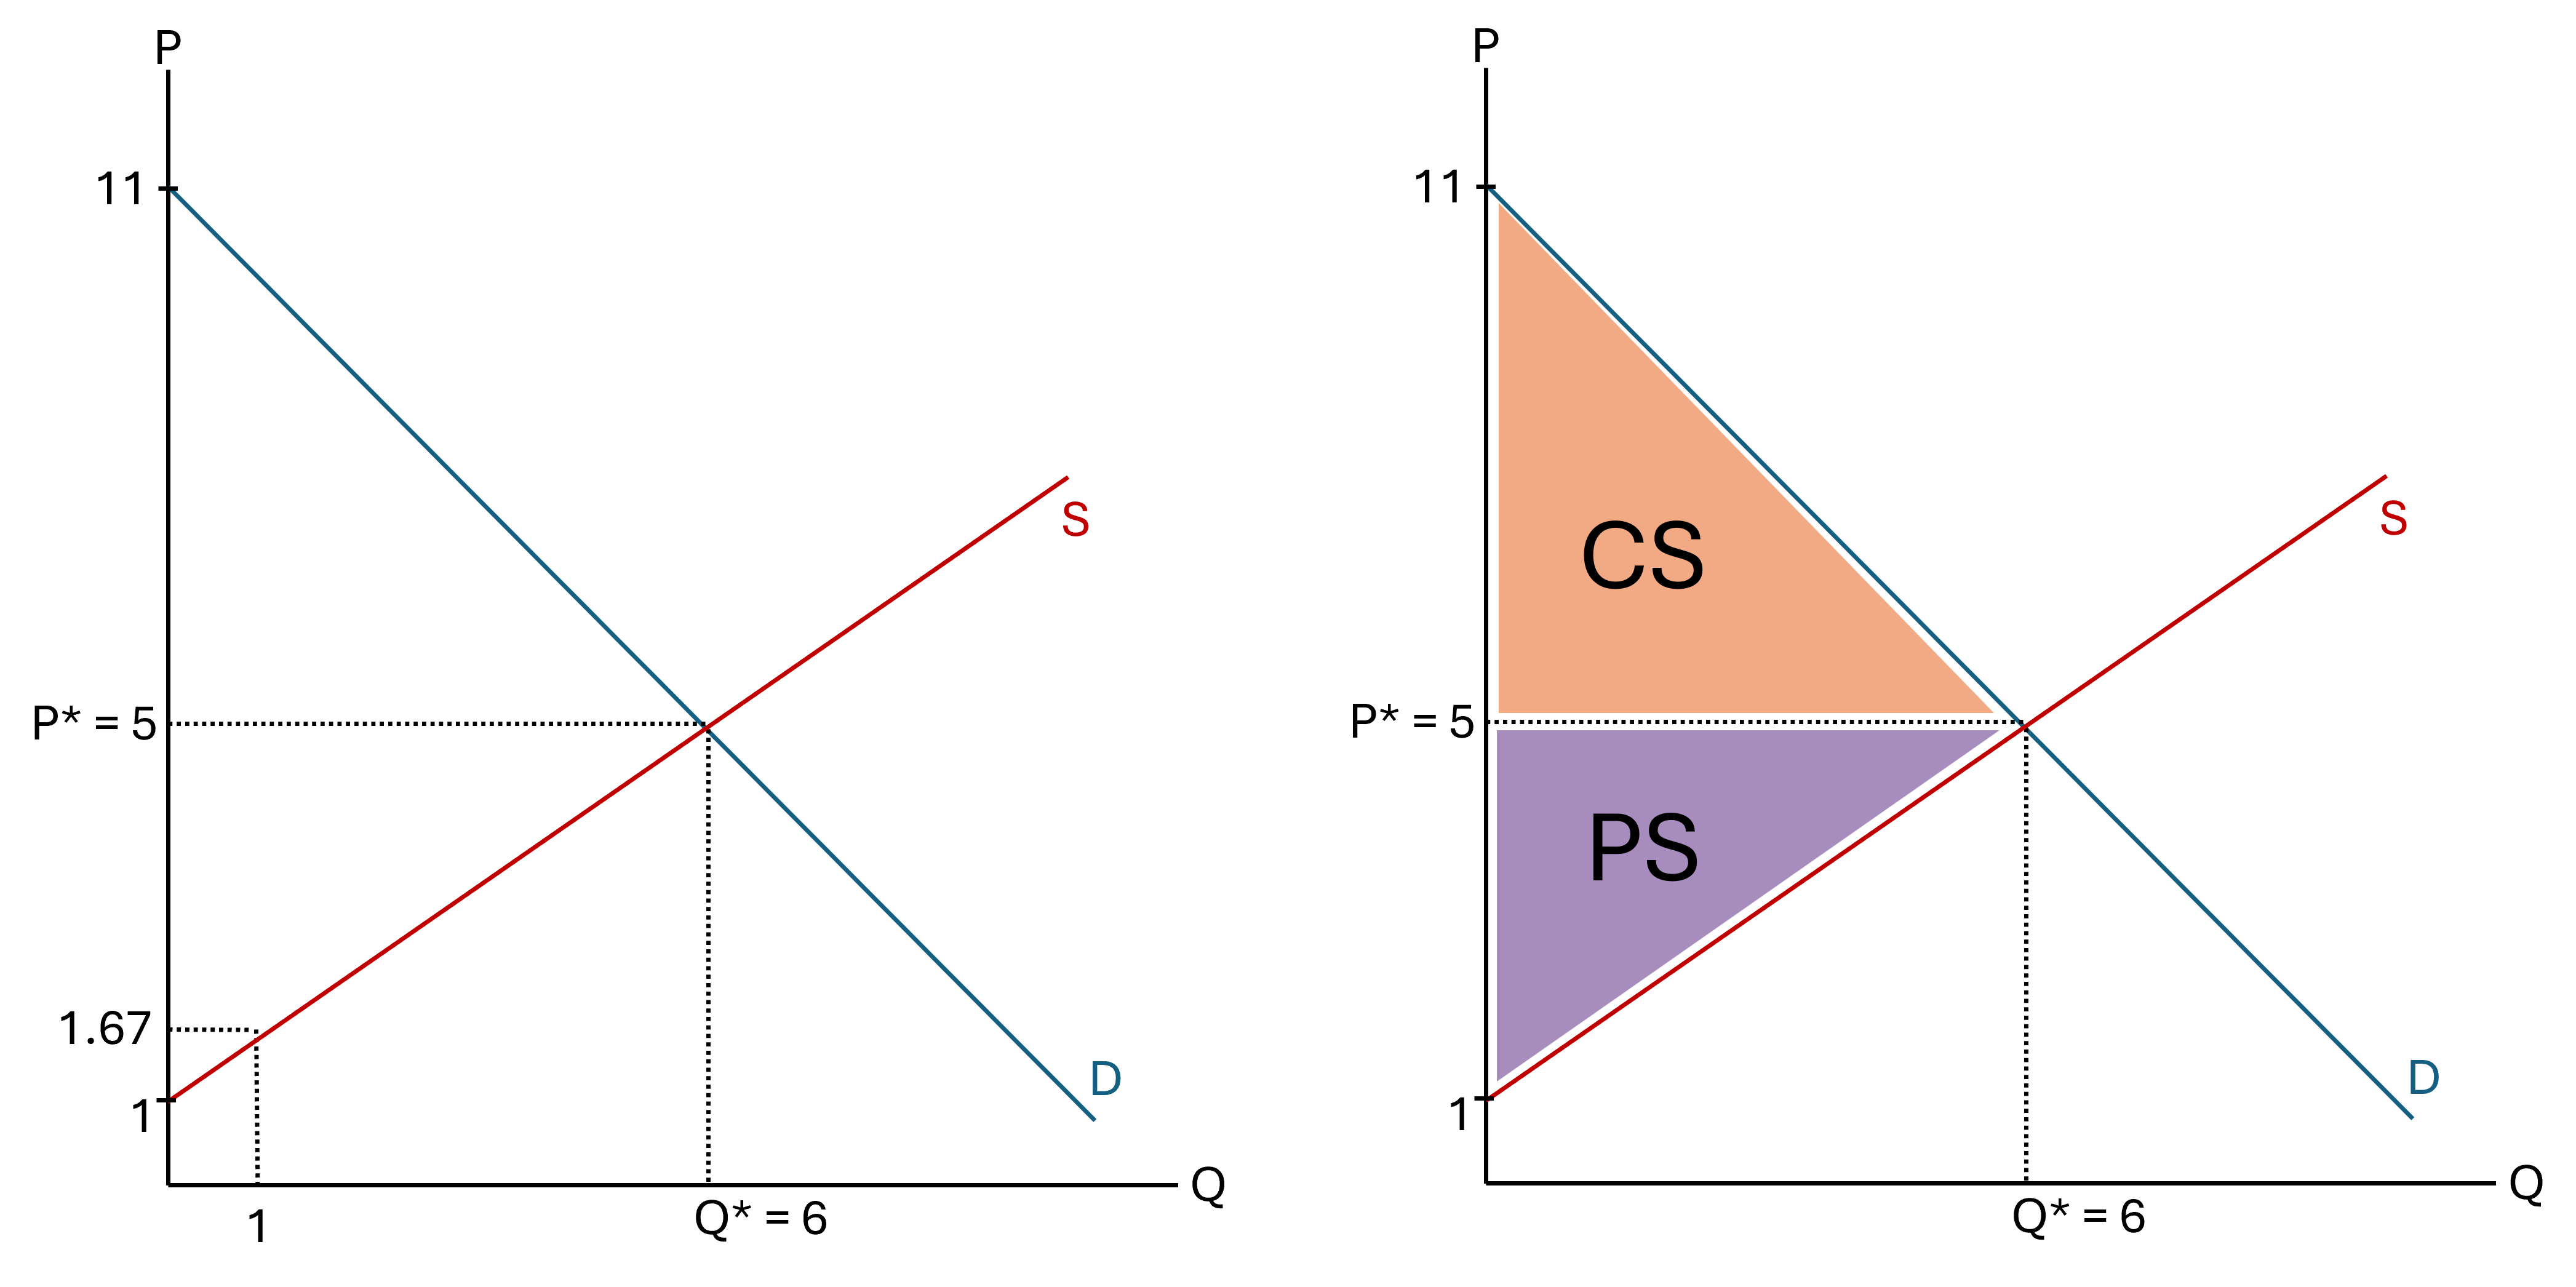
\includegraphics[width=0.85\linewidth]{Picture3.png}
    \end{figure}
    \begin{itemize}
        \item This producer is willing to sell one unit for \$1.67, so he receives \$5 - \$1.67 = \$3.33 of surplus from that unit.
        \item Summing across all units, $PS = \frac{1}{2}bh = \frac{1}{2}(6)(4) = 12$.
    \end{itemize}
\end{frame}

\begin{frame}{Exercise 1: Consumer \& Producer Surplus}
    Consider the market for Boston College Doug Flutie jerseys: 
    \begin{itemize}
        \item[-] $Q^D = 250 - P$
        \item[-] $Q^S = 2P - 50$
    \end{itemize}
    \begin{enumerate}
        \item Find the market equilibrium.
        \item Calculate the consumer surplus, producer surplus, and total surplus.
    \end{enumerate}
\end{frame}

\begin{frame}{Exercise 1: Consumer \& Producer Surplus}
    Solution: 
    \begin{enumerate}
        \item Market equilibrium price and quantity: $P^*=100$, $Q^*=150$
        \vspace{5pt}
        \item $CS = \frac{1}{2}(150)(250 - 100)=\frac{1}{2}(150)(150) =$ 11,250\\
        \vspace{5pt}
        $PS = \frac{1}{2}(150)(100 - 25) = \frac{1}{2}(150)(75) =$ 5,625\\
        \vspace{5pt}
        $TS = CS + PS =$ 16,875
    \end{enumerate}
\end{frame}

\begin{frame}{Welfare Effect of a Tax}
    \begin{itemize}
        \item We know a tax raises the buyer's price, lowers the seller's price, and reduces quantity.\\
        $\implies \:$ Shrinks the CS and PS triangles
    \end{itemize}
    \begin{figure}
        \centering
        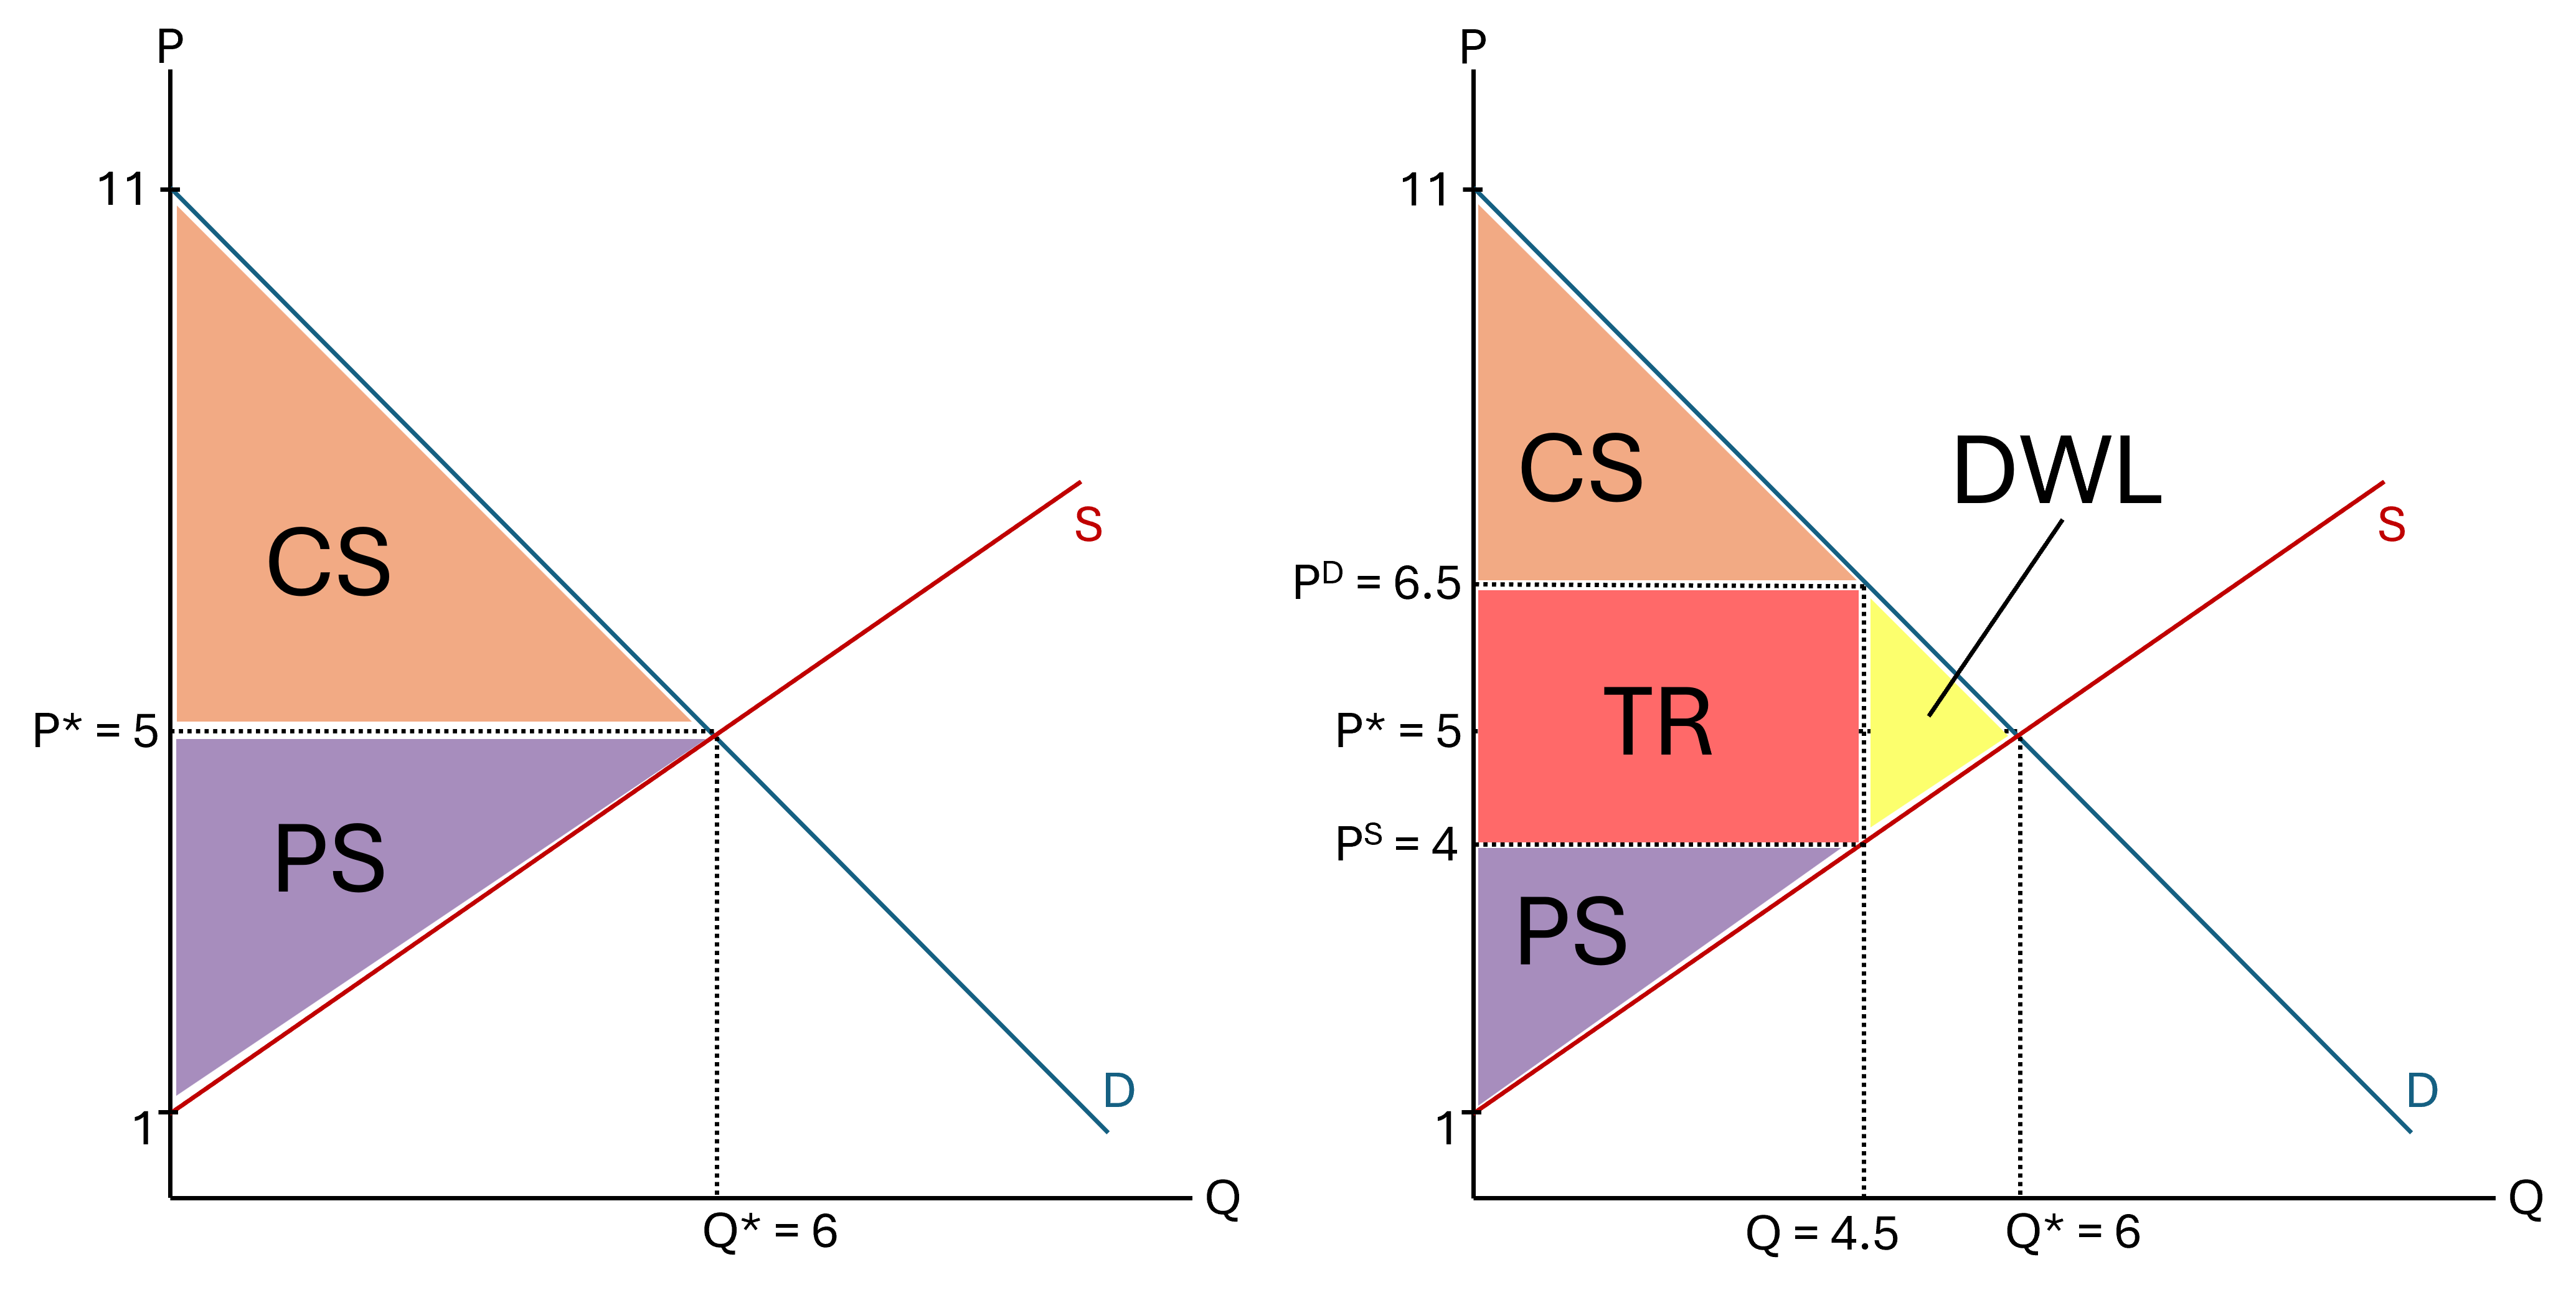
\includegraphics[width=0.85\linewidth]{Picture4.png}
    \end{figure}
    \begin{itemize}
        \item Some CS and PS is converted to tax revenue: $TR = t \times Q$
        \item \textbf{Deadweight Loss} is the CS and PS that is simply lost due to the fall in quantity.
    \end{itemize}
\end{frame}


\begin{frame}{Exercise 2: Welfare Effect of a Tax}
    Suppose a market is described by the following supply and demand equations:
    \begin{itemize}
        \item[-] $Q^D = 200-P$
        \item[-] $Q^S = 2P-100$
    \end{itemize}
    \begin{enumerate}
        \item Find the original equilibrium $P^*$ and $Q^*$.  Calculate Consumer Surplus and Producer Surplus.
        \vspace{5pt}
        \item Suppose the government imposes a tax of \$30 per unit.  
        \vspace{5pt}
        \begin{enumerate}[a]
            \item Find the new $P^S, P^D$ and $Q$.
            \vspace{5pt}
            \item Calculate CS, PS, Tax Revenue, and Deadweight Loss.
        \end{enumerate}
    \end{enumerate}
    \vspace{1in}
\end{frame}

\begin{frame}{Exercise 2: Welfare Effect of a Tax}
Solution:
    \begin{enumerate}
        \item $P^* = 100, \: Q^* = 100$\\
        \vspace{5pt}
        $CS = \frac{1}{2}(100)(100) =$ 5,000\\
        \vspace{5pt}
        $PS = \frac{1}{2}(100)(50) =$ 2,500
        \item 
        \vspace{5pt}
        \begin{enumerate}[a]
            \item $P^S = 90, \: P^D = 120, \: Q = 80$
            \vspace{5pt}
            \item $CS = \frac{1}{2}(80)(80) =$ 3,200\\
            \vspace{5pt}
            $PS = \frac{1}{2}(80)(40) =$ 1,600\\
            \vspace{5pt}
            $TR = (30)(80) =$ 2,400\\
            \vspace{5pt}
            $DWL = \frac{1}{2}(20)(30) = 300$
        \end{enumerate}
    \end{enumerate}
\end{frame}

\begin{frame}{Optimal Taxation}
    \begin{itemize}
        \item A reasonable goal when designing tax policy might be to minimize DWL.\\
        $\implies \:$ Tax goods with inelastic demand or supply.
    \end{itemize}
    \begin{figure}
        \centering
        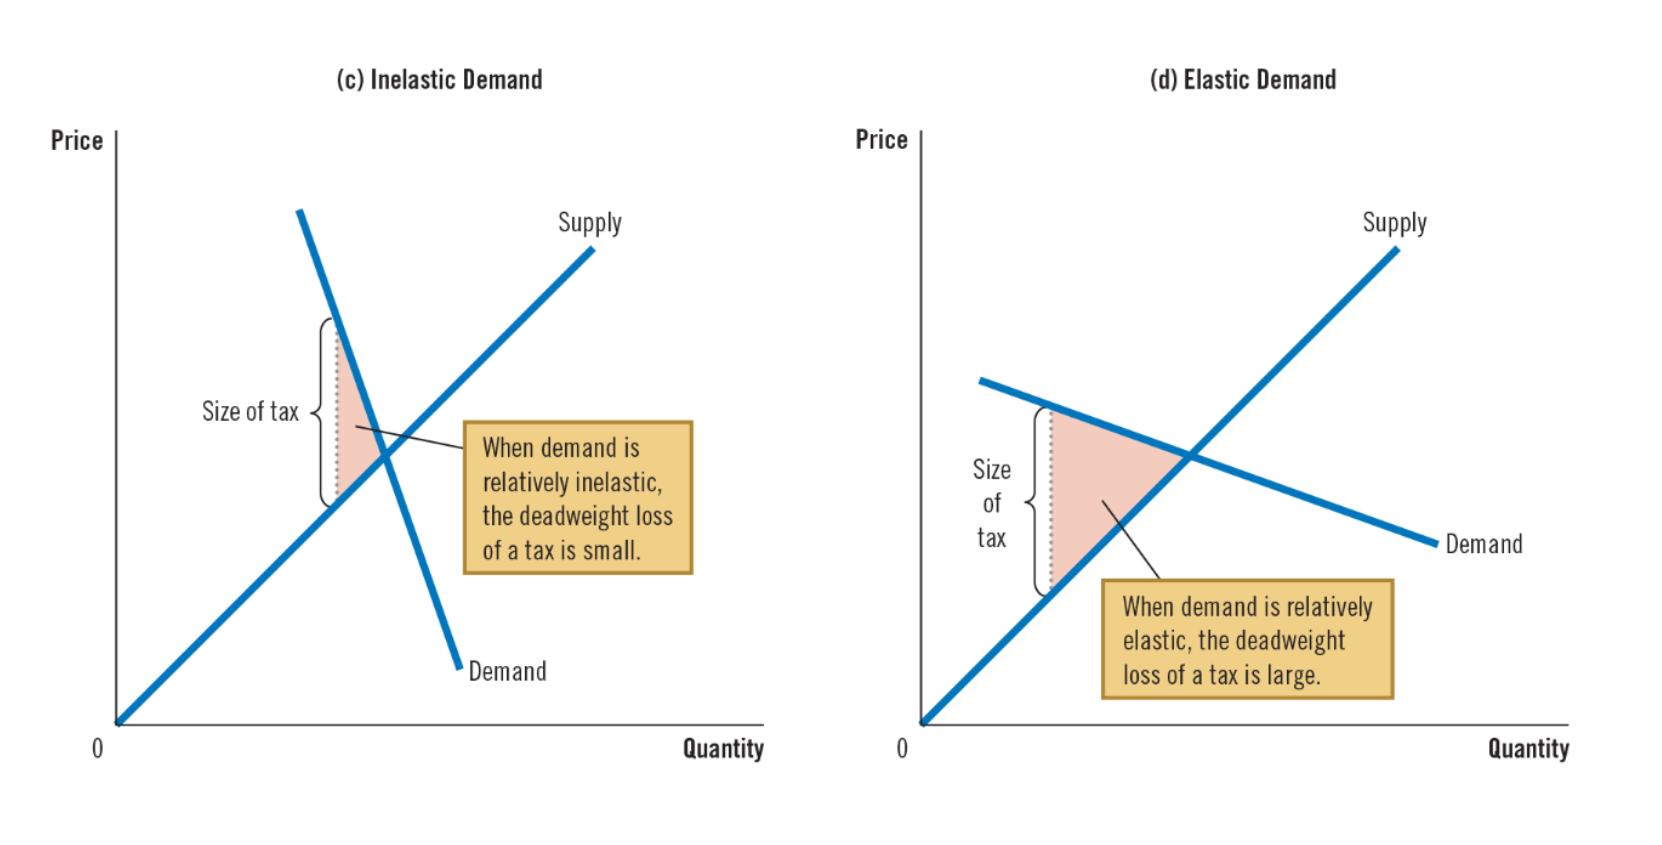
\includegraphics[width=0.8\linewidth]{elasticity_and_dwl.png}
        \caption{Mankiw, Principles of Economics 10th Edition, Chapter 8}
    \end{figure}
    \begin{itemize}
        \item But what kinds of goods tend to be inelastic?
        \item How do we balance DWL minimization with other considerations?
    \end{itemize}
\end{frame}

\begin{frame}{Optimal Taxation: Continued}
    \begin{itemize}
        \item Another goal of tax policy might be to maximize tax revenue.
        \item Economist Arthur Laffer famously brought the tax revenue curve to the public eye after sketching it on a napkin during a meeting with Dick Cheney and Donald Rumsfeld in 1974.
    \end{itemize}
    \begin{figure}
        \centering
        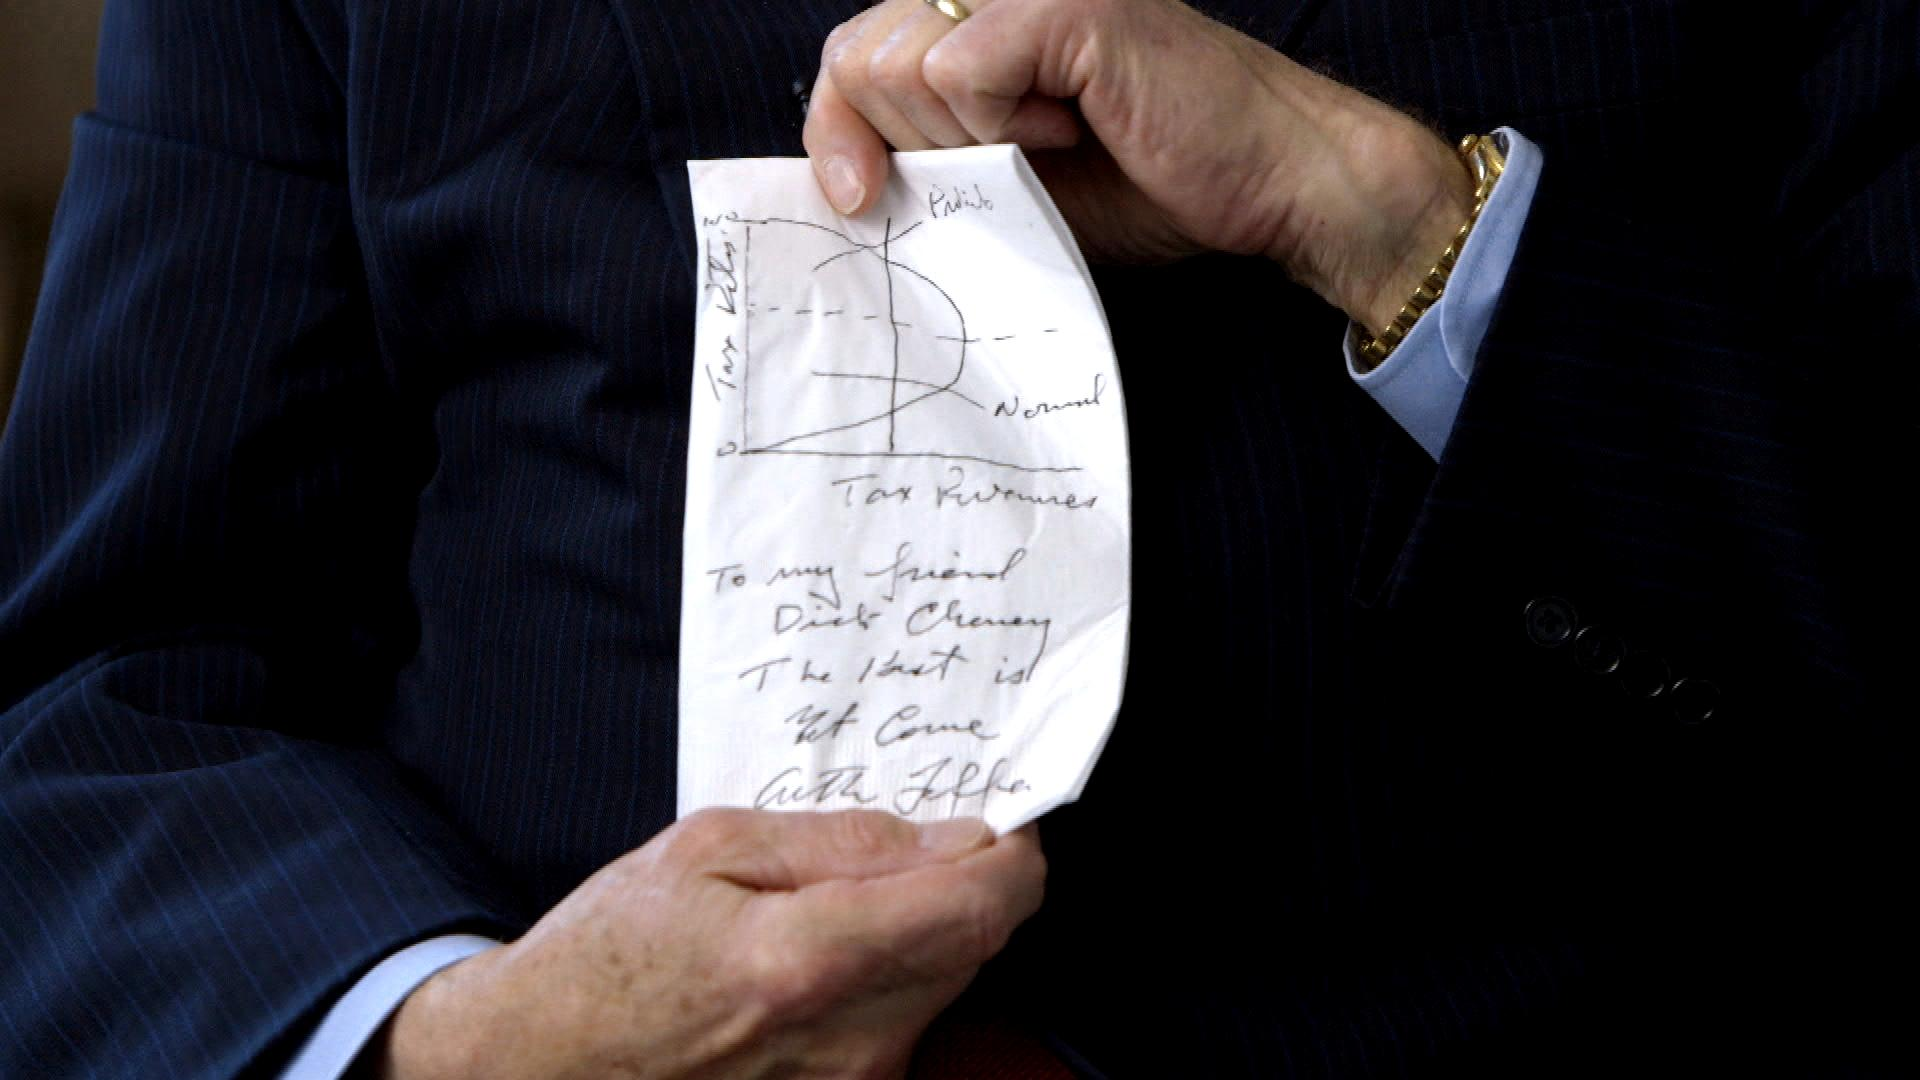
\includegraphics[width=.85\linewidth]{laffer curve.jpg}
    \end{figure}
\end{frame}

\begin{frame}{The ``Laffer Curve''}
    \begin{itemize}
        \item We can derive the Laffer Curve with our `Econ 101' technique!
    \end{itemize}
    \vspace{5pt}
    \begin{itemize}
        \item[-] $Q^D = 200-P$
        \item[-] $Q^S = 2P-100$
    \end{itemize}
    \vspace{10pt}
    \begin{itemize}
        \item Just need to solve for tax revenue as usual, but leave $t$ unspecified:
        \vspace{5pt}
        \item $TR = -\frac{2}{3}t^2 + 100 t$
    \end{itemize}
\end{frame}

%%% OPTIONAL THIRD EXERCISE %%%%%%%%%%%%%%%%%%%%%%%%%%%%%%%%%%%%%%%%%%%%%%%%%%%%%%%%%%%%%%%%%%%%%%%%%%%%%%

% \begin{frame}{Exercise 3: Optimal Taxation}
%     Suppose a market is described by the following supply and demand equations:
%     \begin{itemize}
%         \item[-] $Q^D = 200-p$
%         \item[-] $Q^S = 2p-10$
%     \end{itemize}
%     \begin{enumerate}
%         \item Suppose the government imposes a tax of \$3 per unit. Calculate the consumer surplus, producer surplus, and deadweight loss.
%         \item Suppose the government is considering increasing the tax to \$6 per unit. Should the government increase the tax if 
%         \begin{itemize}
%             \item[-] the government wants to increase tax revenue;
%             \item[-] the government wants to increase the total surplus.
%         \end{itemize}
%     \end{enumerate}
%     \vspace{1in}
% \end{frame}

% \begin{frame}{Exercise 3: Optimal Taxation}
%     \begin{enumerate}
%         \item Without tax: the equilibrium quantity is 130\\
%         With tax: the price paid by consumers is \$72, the price received by producers is \$69, and the equilibrium quantity is 128. \\
%         $CS=0.5\times (200-72)\times 128=8192$, $PS=0.5\times (69-5)\times 128=4096$, $DWL=0.5\times (130-128)\times 3=3$
%         \item With \$3 tax: tax revenue is $3\times 128=384$\\
%         With \$6 tax: the price paid by consumers is \$74, the price received by producers is \$68, the equilibrium quantity is 126, and the tax revenue is $6\times 126=756$.\\
%         To increase tax revenue, the government should increase the tax. However, if the government wants to increase the total surplus, it shouldn't increase the tax as the deadweight loss is larger ($DWL=0.5\times (130-126)\times 6=12$). 
%     \end{enumerate}
% \end{frame}

\end{document}

